% ===== RUBRIC OF TEACHER'S JOB ASPECTS =====

% A single rubric criterion
\newcommand{\rubriccriterion}[4]{
\stepcounter{rubricquestion}
\section*{\therubricquestion: #1}

\smallskip
\note{Unaware:} #2

\note{Beginner:} #3

\note{Guru:} #4

\medskip
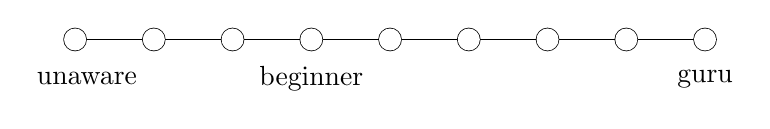
\begin{tikzpicture}
\draw (0,0) -- (8,0);
\foreach \i in {0,1,...,8} % numbers on line
{
\fill[black] (\i,0) circle (1.5 mm);
\fill[white] (\i,0) circle (1.4 mm);
}
\node at (0.15, -0.5) {unaware};
\node at (3, -0.5)    {beginner};
\node at (8, -0.5)    {guru};
\end{tikzpicture}
}

\restoregeometry
\chapter*{Teacher evaluation rubric}
\label{rubric}

The following pages present a rubric for evaluating teaching skills. Many teachers (beginners and veterans alike) don't perceive all the different levels and dimensions of the art of teaching. This often happens because they don't see these skills in others. After months or years of teaching, there may come a moment when you realize that the space for improvement is much larger than you expected\punct{.}\footnote{More information can be found, for example, in the book \emph{How Learning Works: Seven Research-Based Principles for Smart Teaching}.}

\section*{What is an evaluation rubric?}

An evaluation rubric is a self-assessment tool helping you see and describe your knowledge, skills, and abilities. Firstly, it helps you perceive and name all the fundamental parts of a concept (e.g., being able to program means being able to design an algorithm, work with memory effectively, know the syntax, \dots). Secondly, it enables you to evaluate your competence in these parts (e.g., I'm able to design a working algorithm, though I find it problematic to express it in code and I don't optimize memory usage at all).

\section*{How to use the teacher evaluation rubric?}

Fill in the rubric at the beginning of the semester (indicate the level of your skill on the scale). Choose 1--3 areas for you to focus on this semester. If you want to be thorough, try to think of some specific actions to do and appropriate indicators of your progress. Go over the rubric again at the end of the semester and reevaluate your progress in the individual areas.

Another option is to treat the rubric as a manifesto -- the \enquote{guru} descriptions represent our view of the skills great teachers have. We would like to cultivate these in the novice teachers as well.

\newcounter{rubricquestion}

\newpage
\rubriccriterion{Lesson aims and objectives, conscious attention}
{My lessons don't have explicitly set aims/objectives. When teaching, I'm unaware of the current situation or direction. I~often feel lost.}
{Sometimes I see my current aim/objective and I understand effects of the methods I'm using at that moment. However, I'm usually not consciously paying attention to my teaching.}
{I'm almost always paying attention to what aims/objectives I follow, what happens to me and the class, what I'm doing, and what effects it'll have. I know how we arrived at the current situation.}

\rule{\textwidth}{0.4pt}
\rubriccriterion{Class interaction, asking questions}
{I don't interact with the class. I don't ask since I would probably not get answers. I don't know how to engage students.}
{I know it's possible to interact with the class and I~know the tools to do it. Nevertheless, I'm unable to use them well. Sometimes when I ask, I don't get answers.}
{I interact with the class often and do it in a way that engages the students. I can effortlessly solve the situations when I'm not getting answers (e.g., by question reformulation).}

\newpage
\rubriccriterion{Lesson structure}
{I don't think about the lesson structure.}
{I understand the advantages of having a clear structure in the lesson. Despite my attempts, I often get confused or handle too many things at the same time, and students get lost.}
{My lessons have a clear structure. Students know what is happening, what follows next and they see the connections. I~explicitly announce transitions between individual blocks.}

\rule{\textwidth}{0.4pt}
\rubriccriterion{My feelings and satisfaction}
{I'm dissatisfied with my lessons or I do not reflect on my emotions/satisfaction with the lessons. I don't look forward to teaching.}
{I often don't feel confident during the lessons. Sometimes I'm happy about some parts of the lesson, but I often feel tense or afraid of messing up.}
{I feel relaxed and self-confident when teaching. I enjoy it and have my own teaching style.}

\newpage
\rubriccriterion{Formative feedback}
{I do not think about giving personal feedback.}
{I try to give personal feedback to students to help them grow. Nevertheless, I think I'm not doing it often enough or effectively enough. Students don't always see my input as supportive and respectful.}
{I interact with students regularly to give them formative feedback. They know their strengths and weaknesses and see the ways to improve. They feel I respect them and are not afraid of getting feedback.}

\rule{\textwidth}{0.4pt}
\rubriccriterion{Giving instructions and assigning tasks}
{I do not think about the way I give instructions or assign tasks at all.}
{When I give instructions or assign a task, students occasionally don't understand what to do, where to start or what the result should be.}
{When I give instructions or assign a task, students understand what to do and where to start and work towards the result matching my aim.}

\newpage
\rubriccriterion{Diversity and innovation in lesson design}
{I teach the way I was instructed, or I copy the teaching I experienced myself. I don't consider any alternatives.}
{I'm aware one could employ activities of different types to teach. Nevertheless, I don't know many of them, can't introduce them effectively or am unsure why to use them.}
{I know plenty of different activities and design my lessons to achieve variety. The selected activities effectively teach/practice what I intend to. They also engage students in class and increase their motivation to learn.}

\rule{\textwidth}{0.4pt}
\rubriccriterion{Broader context of my lessons} 
{I don't think about the broader context of my sessions and the course.}
{It's difficult for me to explicitly name the knowledge, skills, and abilities I'm teaching. I don't know where these may be useful. I'm unable to see interconnections to other courses.}
{I have a thorough understanding of my teaching aims/objectives. I~know why I'm concentrating on these particular skills and where they will be useful. I can see the bigger picture.}
\vspace*{-1em}

\newpage
\rubriccriterion{Effective explaining}
{I do not reflect on the way I explain things.}
{When explaining something, I'm routinely doubtful if my explanations are useful (help students' understanding).}
{When explaining a theory, I demonstrate solutions and effectively highlight mistakes. I'm able to see things from the students' perspective. My explaining effectively helps students' understanding. I do not explain things unrelated to students' questions.}

\rule{\textwidth}{0.4pt}
\rubriccriterion{Learning environment, teaching systems}
{I don't think about the classroom atmosphere. I don't see systems in my lessons.}
{I tend to think about the policy and atmosphere in the class. I take over particular procedures and strategies (e.g., scoring) from others. Nevertheless, I don't see their effects or don't know how to adjust them.}
{I'm able to create a productive learning environment. I~see the effects of the particular procedures and strategies I use (e.g., scoring, rewards, rituals). I don't take systems over blindly -- I understand their effect and adjust them appropriately.}

\newpage
\rubriccriterion{Flexibility/adjustments on the spot}
{I do not consciously respond to situations arising in the lesson.}
{I am aware of moments where it may be interesting or useful to deviate from the intended lesson plan. Nevertheless, I'm usually unable to react appropriately on the spot.}
{I'm able to adjust my lessons on the fly according to the situation and students' needs. I know enough tools and can use them effectively.}

\rule{\textwidth}{0.4pt}
\rubriccriterion{Teacher-student interaction}
{I don't think about teacher-student interaction or counseling at all.}
{I often find myself helpless when interacting with a~single student (e.g., individual exam, counseling). The interaction is not effective, or the student feels threatened.}
{When interacting with a single student (e.g., exam, counseling), I use time effectively. Students appreciate my support and find it useful. I treat students with respect. }

\newpage
\rubriccriterion{Groupwork, group management}
{I find splitting the class into groups useless. I don't think about working in smaller groups.}
{I'm aware of pairwork or groupwork. I anticipate this could be useful, but I'm still looking for a way to use it.}
{I know when to work with the whole group, when with individual students and when with smaller groups. I effectively use groupwork if the situation calls for it. I have groups interact with each other when appropriate.}

\rule{\textwidth}{0.4pt}
\rubriccriterion{Awareness of classroom atmosphere}
{I don't pay attention to the students, I only pay attention to the educational content.}
{I'm aware the group is sending out signals and that it would be useful to understand and use them for effective teaching and learning. Nevertheless, I can only rarely do that.}
{I'm able to see the classroom atmosphere and students' reactions. I~perceive what's moving the group at the given moment (e.g., weariness, enthusiasm, concern).}
